\subsubsection {}
\label{sec:analysis:research:backArch:monolith}

Монолитная архитектура предполагает развёртывание приложения одним файлом (например, WAR фаил) или архивом файлов (например, приложение на Rails), все модули приложения разрабатываются, развёртываются и тестируются одновременно. Обычно при реализации данного подхода, всё приложение использует одну базу данных. На рисунке \ref{sec:analysis:research:arch:back:monolith} представлен пример организации монолитного приложения\cite{microservices:ma}.

\begin{figure}[h]
  \centering
    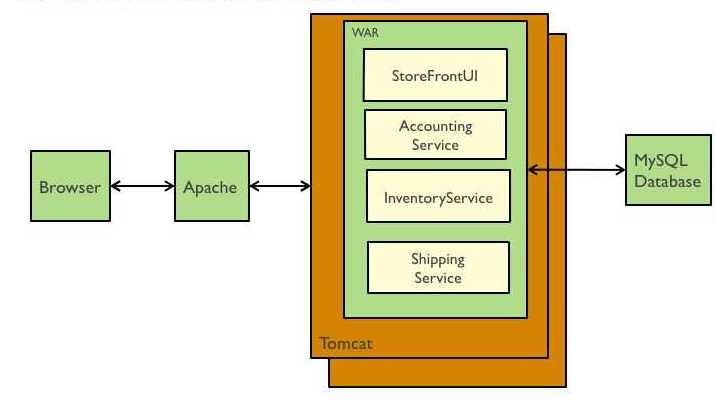
\includegraphics[width=1\textwidth]{inc/img/backend-monolith.jpg}
  \caption{Пример организации монолитного серверного приложения}
  \label{sec:analysis:research:arch:back:monolith}
\end{figure}

К плюсам подхода можно отнести:

\begin{enumerate}
	\item \emph{Простота в разработке} --- целью современных \gls{ide} является поддержка монолитных приложений.
	\item \emph{Простота в развёртывании} --- для старта работы всего приложения нужно лишь запустить один процесс с подготовленным окружением.
	\item \emph{Простота в масштабируемости} --- приложение масштабируется путём запуска дополнительных процессов приложения, организованных при помощи балансировщика нагрузки.
\end{enumerate}

Данный подход удобен до определённого размера приложения, однако, чем больше и сложнее становится приложение, тем существенней становятся следующие проблемы:

\begin{enumerate}
	\item \emph{Сложность поддержки} --- с увеличением кодовой базы, увеличивается сложность ввода нового специалиста в проект. Результатом является общее замедление разработки и отсутствие возможности быстро ускорить разработку при помощи привлечения дополнительных специалистов.
	\item \emph{Перегруженная \gls{ide}} --- хотя современные \gls{ide} и ориентируеются на монолитные приложения, большая кодовая база способна сильно замедлить работу \gls{ide}.
	\item Долгий запуск контейнера приложения.
	\item \emph{Сложности при масштабировании} --- на определённом этапе, в приложении появляются слабые точки производительности. Часто таких точек несколько и они трeбуют разные виды ресурсов (база, процессор, память), однако единственный способ масштабировать приложение --- запускать новый процесс со всем приложением внутри, что не позволяет точечно устранять проблемы.
	\item \emph{Привязанность к технологическому стеку} --- монолитное приложение крайне сложно постепенно переводить на новый технологический стек, а единовременное полное портирование приложения -- опасный процесс, производящий огромное количество ошибок.
\end{enumerate}